\label{first part}
Arimaa is played on a board composed of 64 tiles, similar to a chess board. Like Chess, there are 6 types of pieces, instead they are totally different from those in Chess. From weakest to strongest, they are: rabbits (8 per player), cats, dogs, horses (2 of each per player), camels and elephants (one of each per player).%grammar

\begin{figure}[!h]
\centering

\includegraphics[width=\textwidth]{1_Presentation/1.1_Arimaa_rules_Gabriel/Pictures/Pieces.png}
\caption{The different piece types in Arimaa.}
\label{fig:pieces}
\end{figure}

Each player, starting with the gold player, places all of ones pieces on the two back rows of ones respective side. Then, the gold player plays the first turn.
On ones turn, each player disposes of four moves. One can use these moves on a single piece, or on as many pieces as they desire.

All pieces can move on an adjacent square (but not diagonally), except for the rabbit which cannot move backwards.
A piece can instead use two moves to push or pull a weaker adjacent enemy piece, as shown in figure \ref{fig:displace}.

\begin{figure}[!h]
\centering
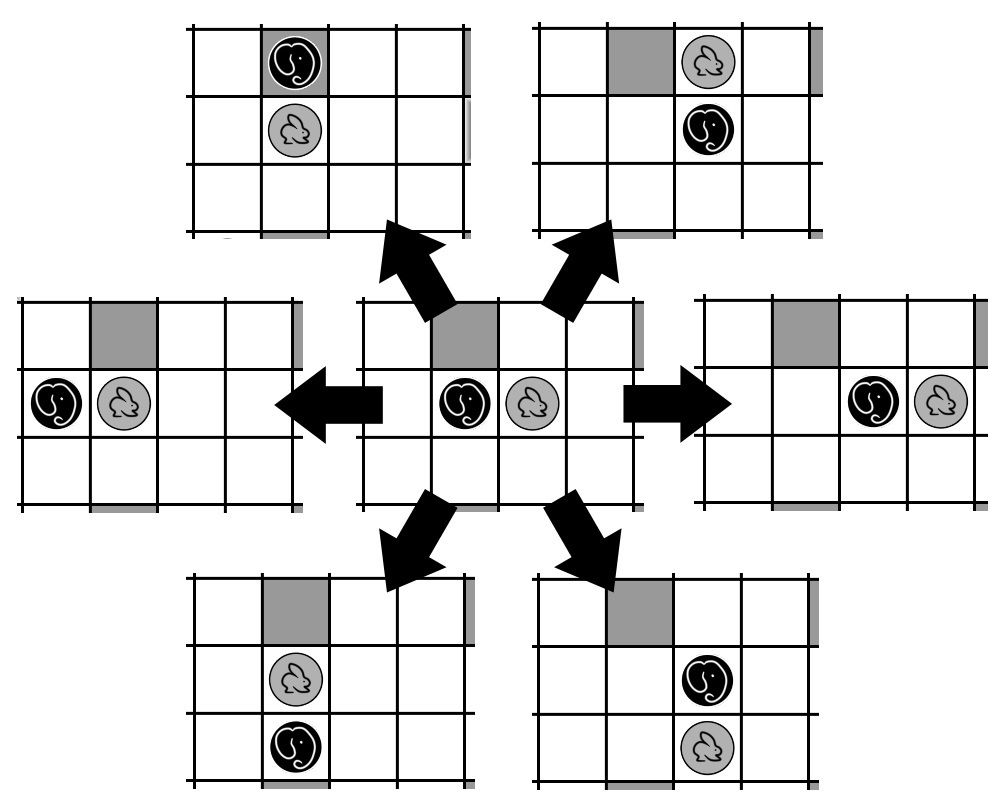
\includegraphics[width=0.6\textwidth]{1_Presentation/1.1_Arimaa_rules_Gabriel/Pictures/Displace.png}
\caption[The different ways of pushing or pulling a weaker enemy piece.]{The different ways of pushing or pulling a weaker enemy piece. Here the elephant pushes or pulls the rabbit.}
\label{fig:displace}
\end{figure}

A piece placed adjacent to a stronger enemy piece is frozen. When a piece is frozen, it cannot move. As shown in figure \ref{fig:freeze}, a piece cannot be frozen while there is an ally piece adjacent to it.

\begin{figure}[!h]
\centering
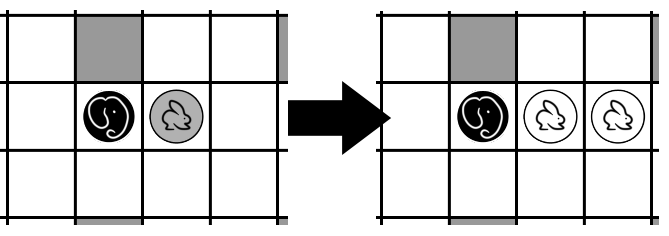
\includegraphics[width=0.5\textwidth]{1_Presentation/1.1_Arimaa_rules_Gabriel/Pictures/Freeze.png}
\caption[Example of the freezing mechanic.]{Example of the freezing mechanic. When the two rabbits are together, the one next to the elephant is no longer frozen.}
\label{fig:freeze}
\end{figure}

There are four traps on the board. As shown in figure \ref{fig:trap}, any piece sitting on a trap with no ally piece next to it dies.

\begin{figure}[!h]
\centering
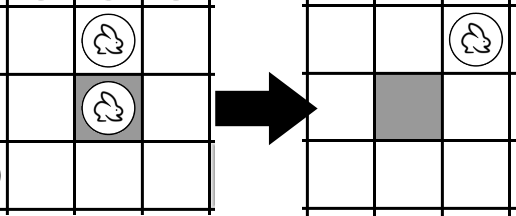
\includegraphics[width=0.5\textwidth]{1_Presentation/1.1_Arimaa_rules_Gabriel/Pictures/Trap.png}
\caption[Example of the traps mechanic.]{Example of the traps mechanic. As soon as there is no other ally pieces adjacent to the rabbit standing on the trap, it dies.}
\label{fig:trap}
\end{figure}

There are four ways to win the game:

\begin{itemize}
\item Victory by reaching the goal: A player wins the game if one of ones rabbits reaches the other end of the board.
\item Victory by elimination: A player wins the game if one eliminates all the rabbits belonging to his opponent.
\item Victory by elimination: A player wins the game if ones opponent cannot make a move on his turn.
\item Victory by repetition: If the same position happens three times in a row, the player that makes it happen the third time loses the game.
\end{itemize}
